\documentclass{report}

\usepackage{graphicx}
\usepackage{listings}
\usepackage{color}
\definecolor{codeColor}{rgb}{0.4, 0.6, 0.8}
\lstset{keywordstyle=\color{codeColor},language=Octave,stepnumber=1,basicstyle=\footnotesize}

\usepackage{enumitem}

\newenvironment{steps}[1]{\begin{enumerate}[label=#1 \arabic*]}{\end{enumerate}}

\makeatletter
\def\step{
   \@ifnextchar[ \@step{\@noitemargtrue\@step[\@itemlabel]}}
\def\@step[#1]{\item[#1]\mbox{}\\\hspace*{\dimexpr-\labelwidth-\labelsep}}
\makeatother

\begin{document}

\title{ Solucion de Ecuaciones No Lineales}
\author{Rub�n Cuadra A01019102}

\maketitle
\begin{abstract}
	Manual de usuario:  'aproxima.m', el objetivo de este texto es documentar la implementacion 2 metodos tales como Interpolacion y metodo del minimo cuadrado para obtener coeficientes de polinomios.
\end{abstract}

\section{Introduccion}
	El codigo consiste en un archivo llamado de la misma manera que la funcion el cual recibe 5 argumentos y nos regresa 2 respuestas y una grafica
\lstinputlisting[ firstline=2, lastline=2]{aproxima.m}

	\textbf{X}  Es un vector ordenado que contiene los componentes x de los puntos por los que pasara el polinomio
	\textbf{Y} Es un vector ordenado que contiene los componentes y de los puntos por los que pasara el polinomio  
	\textbf{N} Es el grado del polinomio que deseamos obtener.
	\textbf{O}  Es una bandera True(1) o False(0),Donde True nos generara el poliniomio por el metodo de minimio cuadrado, mientras que un falso lo obtendra con interpolacion
	\textbf{P} Son una serie de valores en X. Una vez que se obtiene el polinomio se evalua con estos puntos en X 


\section{Comprension del algoritmo}
	
\subsection{Interpolacion}
La interpolacion nos genera un polinomio de grado n donde n = numero de puntos -1. El ejemplo mas claro es cuando uno tiene 2 puntos, se necesitara una recta para unirlos(Grado 1).

\begin{steps}{Paso}
\step Inicializar matriz vacia
\step Iteramos por cada valor en el Vector X
\step Agregamos a la matriz nueva de nxn el vector $xActual^totalDeVectores-iteracionActual$
\step En este punto tendremos una matriz b con 'Resultados' que queremos, despejamos Ax=b y nos dara que los coeficientes(x) = inv(A)*b. Realizamos esta operacion
\step Regresamos los coeficientes

\end{steps}
\subsection{Minimo Cuadrado}
El minimo cuadrado consiste en realizar regresiones a traves de iteraciones para generar una funcion del grado deseado

\begin{steps}{Paso}
\step Obtener la cantidad de vectores en X
\step Generamos un vector b que contenga la Suma de potencias en X por Y(Iteracion hasta grado deseado)
\step Generamos otro vector p que tendra las potencias en X(Iteracion hasta grado deseado)
\step Movemos el Vector p a una matriz denominada A(Iteracion hasta grado deseado)
\step Obtenemos la inv(A)*b ,donde tendremos los coeficientes del polinomio
\end{steps}

\subsection{Aproxima - Grafica}
Despues de obtener los coeficientes por alguno de los dos metodos procedemos a graficar
\begin{steps}{Paso}
\step  Obtenemos un vector ordenado P con los resultados de evaluar los puntos extras en el polinomio generado por los metodos anteriores
\step  Evaluamos el polinomio en intervalos de cada 0.05 , el origen lo define el valor minimo entre el vector X y el vector de puntos extra, asi como el final lo define el maximo de estos mismos
\step Inicializamos un plot que pinte de rojo todo el polinomio, de inicio a fin cada 0.05 lugares
\step A la recta le pintamos los vectores (x,y) que nos dieron en un inicio, de color negro con una X
\step Agregamos los puntos extra que ya evaluamos, se pintan en azul con un *
\end{steps}

Al final se regresan 2 valores,   \textbf{A} ,que es el vector de Coeficientes y  \textbf{E} que nos mandara un 1 si no se puede realizar la interpolacion con el grado de polinomio solicitado

\section{Ejemplo}
Mandamos a llamar la funcion desde un archivo main.m.
Usando los argumentos: 
\lstinputlisting[language=Octave,firstline=1,lastline=5]{main.m}
Llamamos la funcion:
\lstinputlisting[language=Octave,firstline=6,lastline=6]{main.m}
y nos devolveria
\lstinputlisting[language=Octave,firstline=7,lastline=12]{main.m}

\begin{figure} 
    \caption{Grafica del ejemplo.}
    \centering
    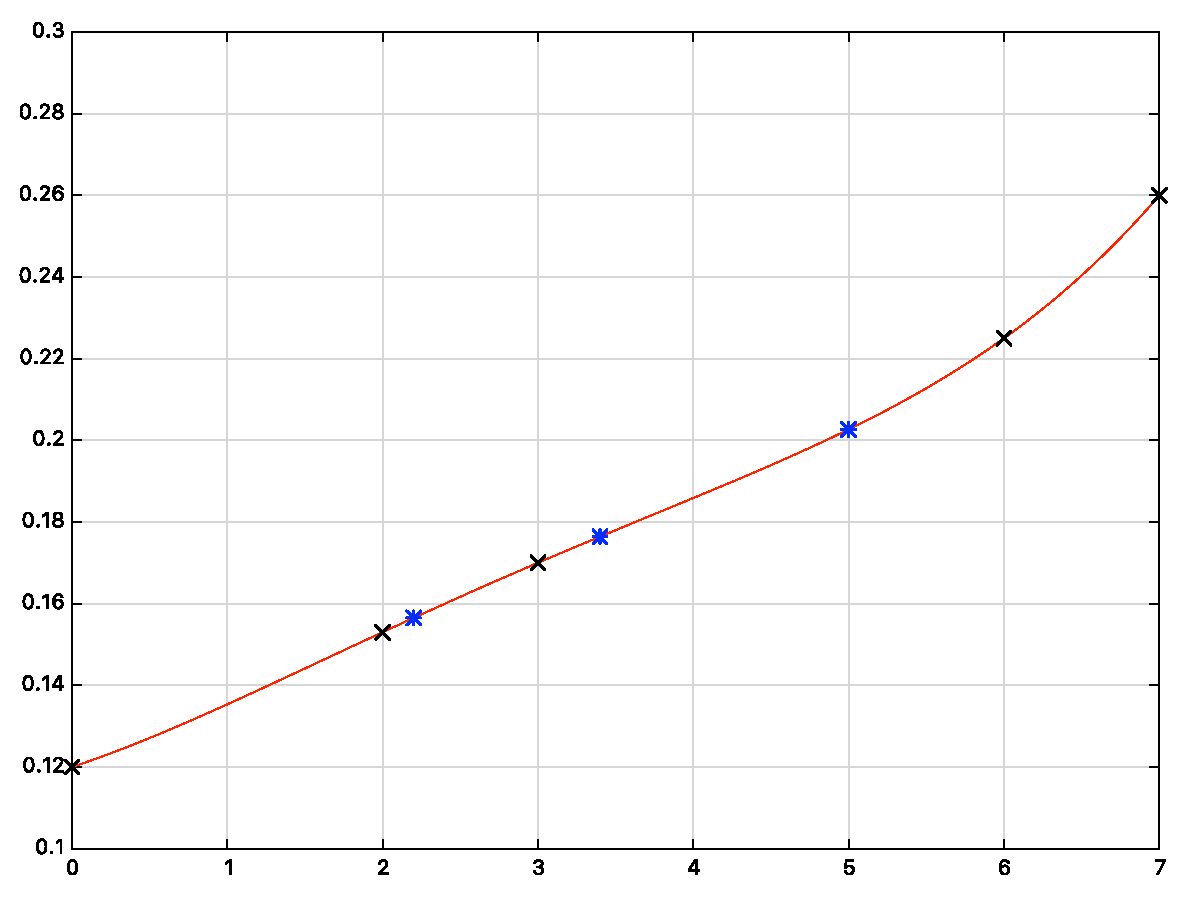
\includegraphics[width=3.5in]{interpol}
    \label{examplefigure}
\end{figure}
\section{Conclusion}
Es un modulo portable que posee varias excepciones, esta facil de implementar y todo bien bien comentado
\footnotetext{Los acentos no se pudieron agregar por cuestion de la codificacion}

\end{document}
